{\footnotesize
\begin{wrapfigure}{r}{0.2\textwidth}
    \raggedleft
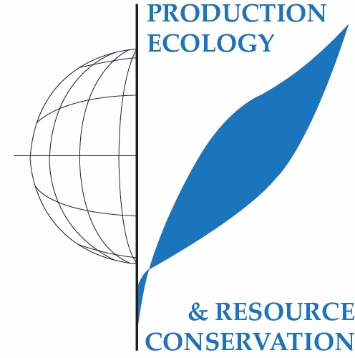
\includegraphics[width=1.61597in,height=1.62917in,alt={A logo of a globe and a wireframe globe Description automatically generated}]{./assets/perc.jpeg.jpg}
\end{wrapfigure}
\textbf{PE\&RC Training and Education Statement}

With the training and education activities listed below the PhD
candidate has complied with the requirements set by the Graduate School
for Production Ecology and Resource Conservation (PE\&RC) which
comprises of a minimum total of 30 ECTS (= 22 weeks of activities)

\textbf{Review/project proposal} \\
- ~~~~Exploring Genetic Progress in Potato \textbar{} 4.5 ECTS

\textbf{In-depth / Topical / On-site Postgraduate Courses} \\
- ~~~~Crop physiology and climate change \textbar{} PE\&RC / University of
  Florida \textbar{} 2019 \textbar{} 2 ECTS \\
- ~~~~Genomic prediction in animal plant breeding \textbar{} WIAS \textbar{}
  2022 \textbar{} 1.5 ECTS

\textbf{Methodological / Statistical Postgraduate Courses} \\
- ~~~~Bayesian Data Analysis \textbar{} PE\&RC \textbar{} 2024 \textbar{}
  1.5 ECTS \\
- ~~~~Matrix Algebra for Engineers \textbar{} Coursera \textbar{} 2020
  \textbar{} 0.5 ECTS \\
- ~~~~Julia Programming Language: From Zero to Expert \textbar{} Udemy
  \textbar{} 2021 \textbar{} 0.5 ECTS \\

\textbf{Invited review of journal manuscripts} \\
- ~~~~Theoretical and Applied Genetics \textbar{} Applied crop genetics
  \textbar{} 2024 \textbar{} 1 ECTS

\textbf{Competence, skills and career-oriented activities} \\
- ~~~~Scientific Integrity \textbar{} WGS \textbar{} 2023 \textbar{} 0.6
  ECTS \\
- ~~~~Writing Week \textbar{} PE\&RC \textbar{} 2023 \textbar{} 1 ECTS \\
- ~~~~Time \& project management \textbar{} Solynta \textbar{} 2022
  \textbar{} 0.4 ECTS

\textbf{Scientific Integrity/Ethics in science activities} \\
- ~~~~Ethics and Animal Science \textbar{} WGS \textbar{} 2023 \textbar{}
  0.8 ECTS

\textbf{PE\&RC Retreat, PE\&RC Day, and other PE\&RC events} \\
- ~~~~PE\&RC weekend for first year PhD candidates \textbar{} 2019
  \textbar{} 0.9 ECTS \\
- ~~~~PE\&RC weekend for last year PhD candidates \textbar{} 2023 \textbar{}
  0.6 ECTS

\textbf{National/local scientific meetings, seminars, and discussion
groups} \\
- ~~~~Book club reading Probability Theory and Statistical Inference by Aris
  Spanos (Discussion over 10 chapters) \textbar{} 2020 \textbar{} 1 ECTS \\
- ~~~~Department book reading of Statistical Principles for the design of
  experiments by Mead, Gilmour, and Mead (15 discussions) \textbar{}
  2023 \textbar{} 1.5 ECTS \\
- ~~~~Literature Discussions over potato related topics with industry
  partner (Two years participation) \textbar{} 2020-2022 \textbar{} 3
  ECTS \\
- ~~~~22\textsuperscript{nd} European Association for Potato Research
  meeting \textbar{} 2024 \textbar{} 1.2 ECTS

\textbf{International symposia, workshops and conferences}\\
- ~~~~21\textsuperscript{st} Eucarpia general congress and potato meeting
  \textbar{} Online due to Covid \textbar{} 2021 \textbar{} 2.2 ECTS
- ~~~~31\textsuperscript{st} Plant \& Animal Genome Conference \textbar{}
  San Diego, USA \textbar{} 2024 \textbar{} 2.8 ECTS

\textbf{Lecturing/Supervision of practicals/tutorials} \\
- ~~~~Statistics 1b Practical \textbar{} 2020 \textbar{} 6 days \textbar{}
  1.8 ECTS \\
- ~~~~Statistics 1a Practical \textbar{} 2021 \textbar{} 6 days \textbar{}
  1.8 ECTS \\
- ~~~~Statistics 1b Practical \textbar{} 2021 \textbar{} 6 days \textbar{}
  1.8 ECTS

\textbf{BSc/MSc thesis supervision} \\
- ~~~~Research topic 1: Novel prediction methods for pre-breeding program in
  potato \textbar{} 3 ECTS
}
